\documentclass[dvipdfmx]{jsarticle}
\usepackage{rsj2011e}
\usepackage{amsmath,amssymb}
\usepackage[usenames]{color}
\usepackage{graphicx}
\usepackage{hyperref}

\hypersetup{% hyperrefオプションリスト
draft=false,
colorlinks=true,%
linkcolor=blue,
citecolor=Brown,
urlcolor=blue
}

\begin{document}
\title{画像システム特論発表用レジュメ}
\author{是松 優作,最上 伸一}

\setlength{\baselineskip}{4.4mm}	% 行間の設定
\maketitle
\thispagestyle{empty}
\pagestyle{empty}

\section{概要}
%「4.アプリケーションを作ってみた」を実施したことを書く.
本稿では,「4.アプリケーションを作ってみた」に基づき,
%実施内容の概要を書く.
与えられた画像からその色境界を識別してクラスタリングすることで,塗り絵の問題を自動生成するアルゴリズムを提案する.

\section{提案手法}
% 課題4の場合は,アプリケーションの目標仕様を1節で述べ,本節では必要とな
% る画像処理とその提案アルゴリズムの詳細を述べる.

塗り絵の問題を自動生成するために,入力画像に2種類の画像処理を施す.
\begin{enumerate}
\item 画像をクラスタリングして色の種類を減らし,塗り絵の模範解答の画像を生成する{\gtfamily クラスタリング処理}.
\item 塗り絵の模範解答画像から,塗り絵の問題を作成する{\gtfamily 境界識別処理}.
\end{enumerate}

\subsection{クラスタリング処理}
塗り絵を行いやすい画像を得るためには,色の類似度・画像の空間的な距離を同時に考慮に入れつつ,
塗り絵に用いる色の種類をある閾値以下に抑えることが望ましい.
そこで本稿では,mean shift 法を用いていくらかの画像クラスタリングを行った後の画像に,
さらに k-means 法をかける手法を提案する.


\subsection{境界識別処理}
上記手法によって得られた正解画像から塗り絵の問題を自動生成するために,
色の一様な部分を白色に,色の境界線を黒色にすることで対象画像を線画化する.


% オープンソースを使用した場合は,その詳細を述べる.また,ソースコードを公
% 開できる場合は,その入手先を記述する.

\subsection{ソースコード}

本手法のソースコードは,

\noindent\url{https://github.com/diesekiefer/ImagingSystem}

\noindent より取得可能である.


\section{実験}

実験の条件を述べる.実験に用いた画像の詳細を述べる.自分で用意した画像の
場合は,カメラの詳細を述べる.計算機の詳細と計算時間を述べる.実験結果の
概要を述べる.

\section{結論}


\begin{figure}[t]
\centering
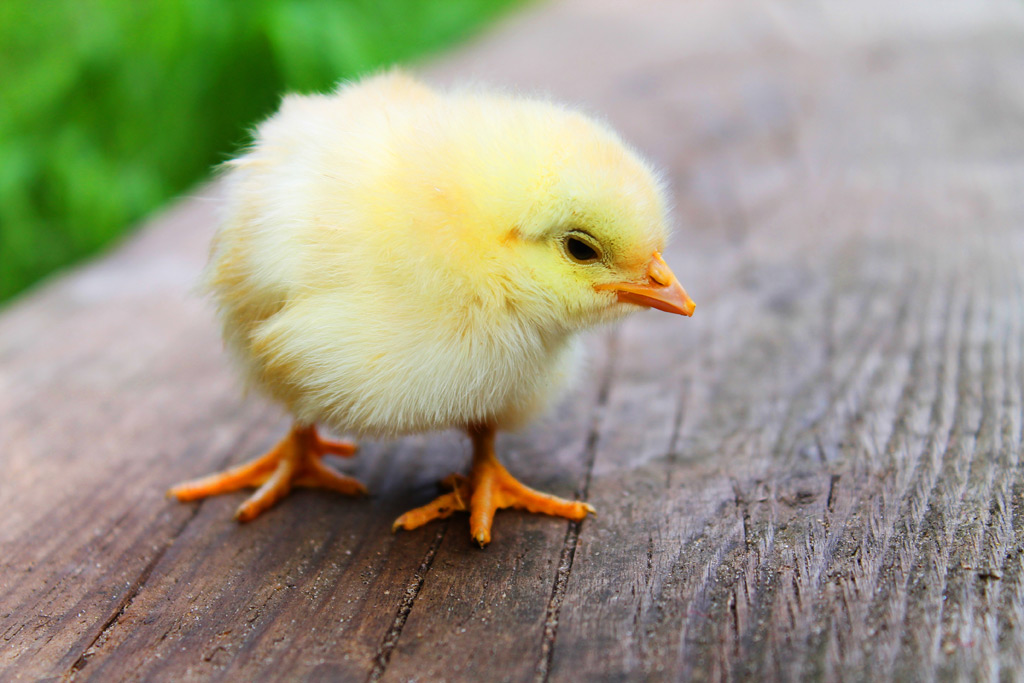
\includegraphics[width=70mm]{hiyoko_PD.png}
\caption{\quad 元画像.}
\label{fig:original}
\end{figure}
\begin{figure}[t]
\centering
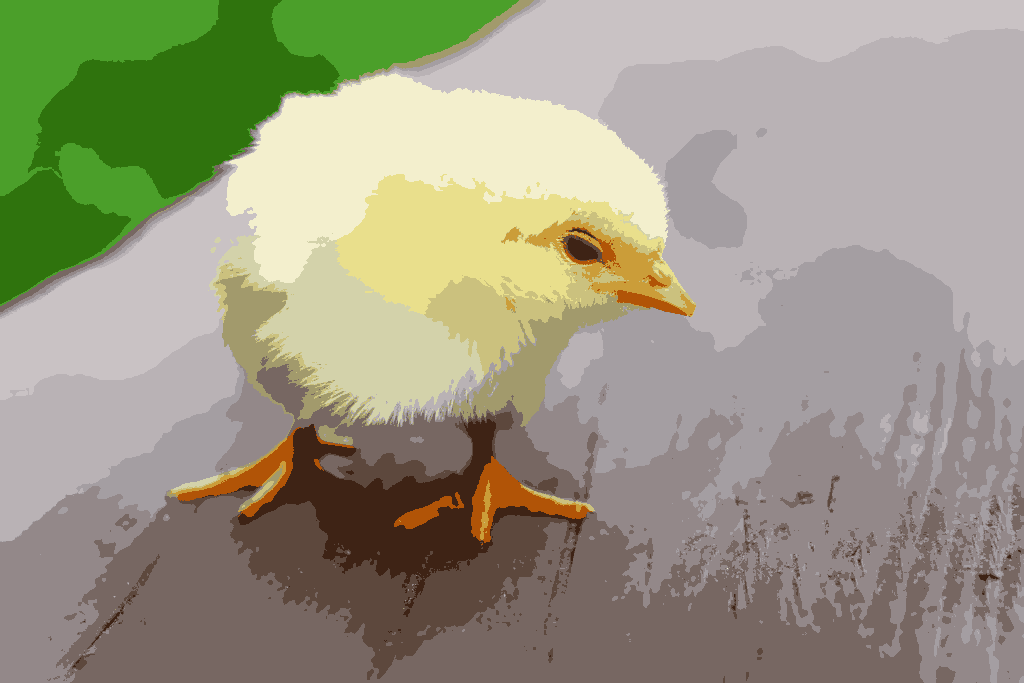
\includegraphics[width=70mm]{hiyoko_16_k-shift.png}
\caption{\quad クラスタリング処理を行った後.}
\label{fig:original}
\end{figure}

% \small
% \begin{thebibliography}{10}
% %%%%%%%%%%%%%%%%%%%%%%%%%%%%%%%%%%%%%%%%%%%%%%%%%%%%%%%%%%%%%%%%%%%%%%%%%%%%%%%
%
% \bibitem{gazo2000}
% 画像太郎, 鈴木一郎:
% ``画像システム特論レジュメの書き方'',
% 日本画像学会誌, vol. 99, no. 4, pp.8-12, 2082.
% \bibitem{website}
% ``画像太郎アルゴリズムのオープンソース'',
% {\tt http:/ /rsj2014.rsj-web.org/}
%
% %%%%%%%%%%%%%%%%%%%%%%%%%%%%%%%%%%%%%%%%%%%%%%%%%%%%%%%%%%%%%%%%%%%%%%%%%%%%%%%
% \end{thebibliography}
% \normalsize
\end{document}
